\section{Method}
In this section we discuss the way in which we process and analyse the data we
obtain from EUMETSAT. First we detail the process of thresholding, which we use
to distinguish between cloud and land pixels. Then, we explain how these
thresholds are used to create useful data products from the raw data.

\subsection{Thresholding}
\label{sec:method:thr}
The most essential part of processing the EUMETSAT images is the ability to
differentiate between cloud and land. Clouds have a much higher reflectance than
land (notable exceptions to this are snow, ice and salt pans) -- if mistakenly
identified as land pixels, they will erroneously skew the value of those pixels
to higher values.

On a clear day any given pixel should have a value that corresponds to that
pixel's ``true'' value (hereafter the \emph{ground} value), with some small
variation contributed by shadows cast by nearby clouds, the variation in
\emph{solar zenith angle} throughout the year, and atmospheric interference
effects. On a cloudy day a pixel's value will be systematically pulled towards
higher than ground values. It follows then that the distribution of a pixel's
value will be bimodal, with the lower peak corresponding to the ground value,
and the large peak corresponding to cloudy values.

The task is then one of producing thresholds that reliably separate the two
peaks. Otsu's method \citep{gonzalez2008} separates pixels into two groups, or
\emph{classes}, by maximising the variance between these classes, making it an
optimum method for thresholding\footnote{We have made use of \texttt{scipy}'s
  Otsu thresholding implementation.}. An example of Otsu thresholding at work is
shown in Figure \ref{fig:otsu} for a random pixel.
\begin{figure}
  \centering
    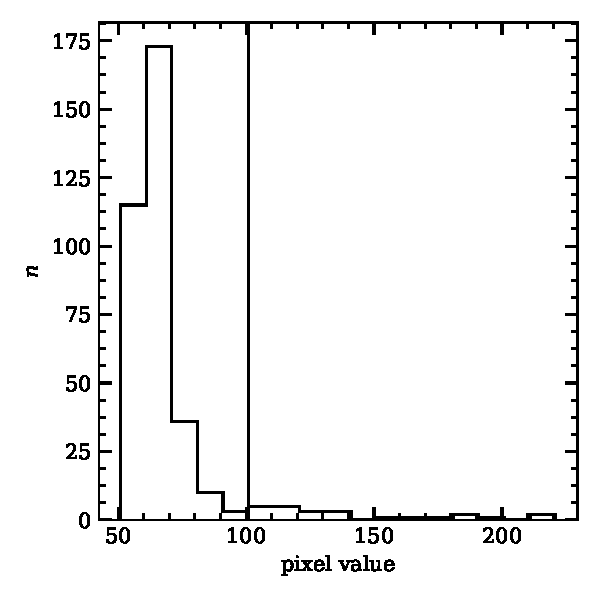
\includegraphics[width=0.8\linewidth]{figures/otsu_bimodal.pdf}
    \caption{The histogram of pixel values for a random pixel. Shown by the
      vertical line is the threshold calculated using Otsu's method -- it can be
      seen how well this method separates the two peaks.}
    \label{fig:otsu}
\end{figure}
All pixels with a value below the threshold will be identified as land and all
pixels with a value greater than or equal to the threshold will be identified as
cloud. Please refer to Section \ref{sec:disc:thresh} for a discussion of
suitable we determined Otsu's method to be in identifying cloud.

Now that we have the method for calculating the threshold of a single
pixel all that remains is to apply it to the entire image, the process for doing
so is detailed in Figure \ref{fig:thr_fc}.
\begin{figure}[t!]
  \centering
  \includegraphics{threshold_flowchart.pdf}
  \caption{Flowchart for calculating threshold values.}
  \label{fig:thr_fc}
\end{figure}

\subsection{Cloud coverage}
Using the thresholds calculated by the method in Figure \ref{fig:thr_fc} we
produce daily cloud masks, which are arrays of the same size as the input image
containing with values of `1' for cloud pixels and `0' for land pixels. For
cloud coverage we use the VIS0.6 and VIS0.8 bands from Table \ref{tab:seviri},
as clouds are brighter in these bands than in the NIR band. From our preliminary
analysis we found that cloud coverage was generally more extensive in the VIS0.6
band, although this was not always the case. To err on the side of caution and
produce a comprehensive cloud mask, we categorised a pixel as cloudy if it is
classified as such in \emph{either} band.

The number of cloud pixels $n_{\mathrm{cloud}}$ for a given day, then, is found
by summing the cloud mask. Cloud coverage is calculated as the ratio of cloud
pixels to total land pixels in the image $N$
\begin{equation}
  \mathrm{CF} = \frac{n_{\mathrm{cloud}}}{N} \,,
  \label{eq:cloud_frac}
\end{equation}
where $N$ is found by summing over all of the land pixels in the land mask for
the given region.

\subsection{Vegetation}

\begin{figure*}
  \centering
  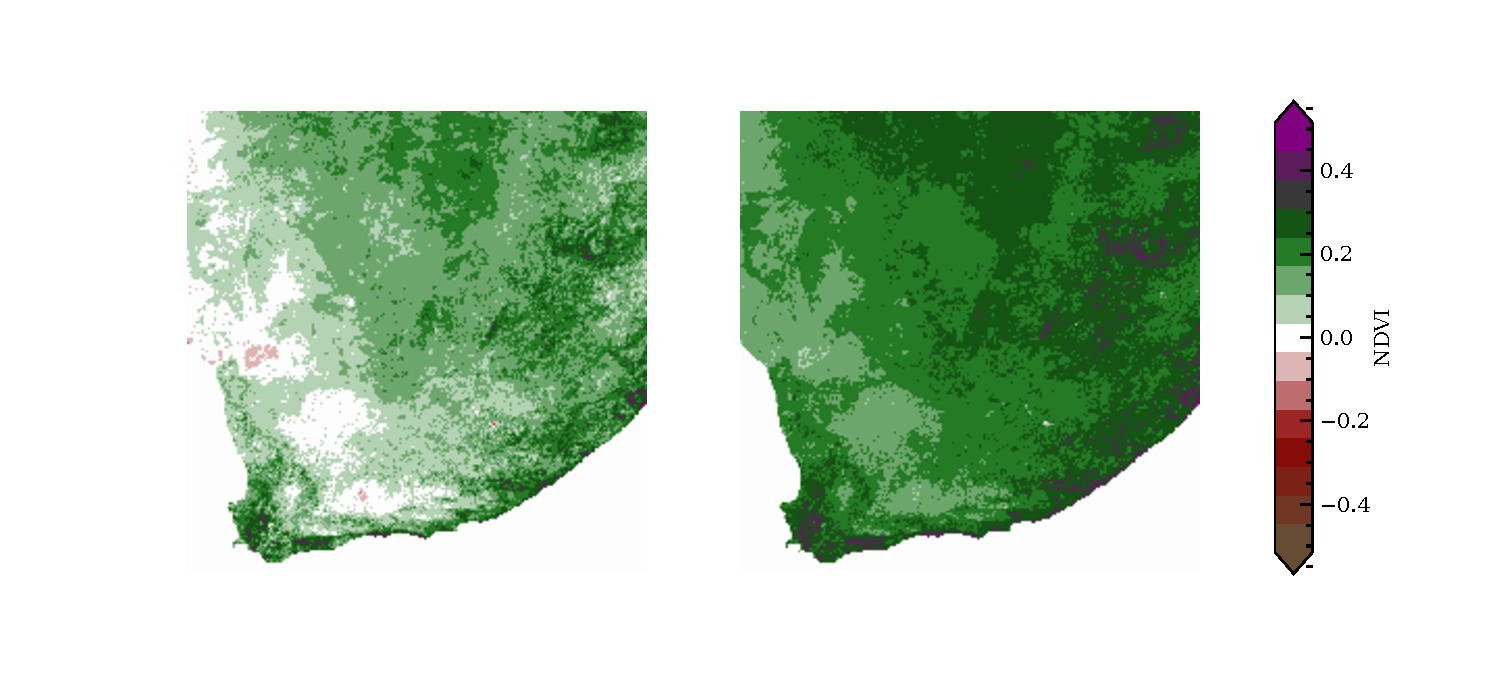
\includegraphics[width=0.85\textwidth]{figures/ndvi_calibration_comparison.pdf}
  \caption{Comparison between NDVI calculated for uncalibrated data (shon left),
    and calibrated data (shown right). The uncalibrated NDVI shows a wider range
    of values, with large areas where NDVI is close to zero (in which case
    $\rho_{\textrm{NIR}}\approx\rho_{\textrm{R}}$), and some regions where NDVI is
    negative. The calibrated NDVI shows neither of these traits, and so we can
    see how using uncalibrated NDVI would lead to erroneous conclusions.}
  \label{fig:calibrationcomp}
\end{figure*}

As described in Section \ref{sec:data:calib} the raw data in the PNG files are
\emph{pixel count} data, \emph{not} radiance data. Before any NDVI calculations
are performed we must calibrate each data channel, so that we have the radiance
data which is required for NDVI. The calibration data is listed in Table
\ref{tab:calibration}. As a matter of interest, a visual comparison of NDVI with
and without calibration is show in Figure \ref{fig:calibrationcomp}. With the
calibrations complete, Equation \eqref{eq:ndvi} is used to calculate the NDVI.

\subsection{Analysis}
\label{sec:analysis}
In order to make useful comparisons with our data products, we need some method
of determining whether a measurement is anomalously large or small in comparison
to some baseline value. The baseline value will generally be a year-long
average, though occasionally the median is a better choice where outliers exist
in the data. 

Weather data are inherently noisy over day-to-day timescales, so first we smooth
the data by taking monthly averages. As can be seen \ref{fig:smoothcomp}, the CF
varies rapidly day-to-day and so obscures any underlying features in the
data. Smoothing that data by averaging over a larger period reduces the daily
variation, leaving the larger trends visible. 

Once we have baseline measurements, we can then calculate the anomalies which
tell us how different a particular measurement is from the average for that time
of year. If $x_{i}$ is the measurement (e.g. NDVI) for a particular month and
year then we define the anomaly as
\begin{equation}
  x_{i\sigma}=\frac{x_{i}-\tilde{x}_m}{\tilde{x}_m}
  \label{eq:anoms}
\end{equation}
where $\tilde{x}_m$ is the median value for that month. The $\tilde{x}_m$ are
defined by calculating the median for each month across the all of the available
years.

Weather patterns like the ENSO vary over a few months or longer, so we are
interested in signals of a similar timescale. To be confident that what were
observing is relevant, and not just transient, we smooth the monthly anomalies
using a five month moving average. Smoothing is done in an efficient way by
using convolution \citep{gorry1990}.

The particular choices for baselines and smoothing parameters in each of our
analyses will be described and justified in more detail in the respective
sections.


%% Local Variables:
%% fill-column: 80
%% TeX-master: "report"
%% End:
